\documentclass[tikz]{standalone}

\usepackage{pgfplots}

\usepackage[utf8]{inputenc}
\usepackage[T1]{fontenc}
\usepackage{times}

\begin{document}

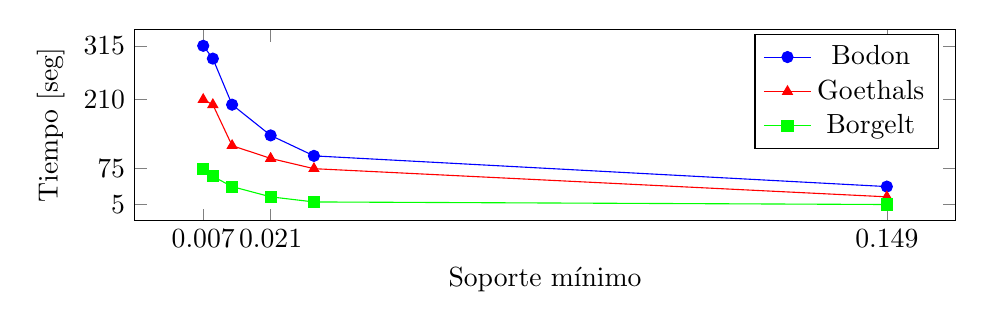
\begin{tikzpicture}
	\begin{axis}[width=12cm,
							height=4cm,
							xtick={0.149,0.021,0.007},
							ytick={5,75,210,315},
							%title={BMS-POS},
							xlabel={Soporte m\'inimo},
							ylabel={Tiempo [seg]},
							xticklabel style={/pgf/number format/.cd,fixed,precision=3}
							]
		\addplot[color=blue,mark=*] coordinates {(0.149,40) (0.030,100) (0.021,140) (0.013,200) (0.009,290) (0.007,315)};
		\addlegendentry{Bodon}
		\addplot[color=red,mark=triangle*] coordinates {(0.149,20) (0.030,75) (0.021,95) (0.013,120) (0.009,200) (0.007,210)};
		\addlegendentry{Goethals}
		\addplot[color=green,mark=square*] coordinates {(0.149,5) (0.030,10) (0.021,20) (0.013,40) (0.009,60) (0.007,75)};
		\addlegendentry{Borgelt}
	\end{axis}
\end{tikzpicture}

\end{document}
